\documentclass{pl-slide}

\usepackage[british]{babel}
\usepackage[british]{datetime2}
\usepackage{ulem}
\usepackage{qrcode}

\usepackage{tikz,calc}
\usetikzlibrary{shapes, shapes, arrows, chains, fit, quotes}

\tikzstyle{trienode} = [draw=text-color, rounded corners]
\tikzstyle{bucket} = [draw=text-color, rectangle]

\definecolor{verystable}{HTML}{13f6e9}
\definecolor{stableenough}{HTML}{ccff00}
\definecolor{unstable}{HTML}{ffa500}

\settheme{neutral-2022}

%Information to be included in the title page:
\title{Effectiveness of Bitswap Discovery Process }
%\subtitle{Our DHT is in good shape!}
\author{Gui Michel}
\avatar{resources/avatar.jpg}
\handle{@guissou}
\group{ProbeLab}
\institute{Protocol Labs}
\event{Engelberg Colo}
\date{\DTMdate{2023-01-11}}

\begin{document}

\frame{\titlepage}

\begin{frame}
\frametitle{Motivation}
\begin{itemize}
	\itemc Measure whether Bitswap is efficient to discover content
	\itemc Bitswap has a \texttt{ProviderSearchDelay} parameter whose value is set to 1 second
	\itemc Get rid of IPFS magic numbers

\end{itemize}
\end{frame}

\begin{frame}
\frametitle{Measurements Setup}
\begin{itemize}
	\itemc Request CIDs collected by sniffing the Bitswap network
	\itemc Bitswap has 15 seconds to find and fetch 1 block
	\itemc Prevent DHT lookup inside Bitswap
	\itemc If Bitswap fails to discover content, verify if content is still available
	\itemc Prevent recursive content resolution
	\itemc Run on a Google Cloud VM in Central Europe
\end{itemize}
\end{frame}

\begin{frame}
\frametitle{Discovery Process Stats}
\begin{itemize}
	\itemc \texttt{98.37\%} discovery success rate (within 15 seconds)
	\itemc On average \texttt{856} distinct remote peers are solicited for each Bitswap request
	\itemc On average \texttt{1714} messages are sent for each Bitswap request
\end{itemize}
\end{frame}

\begin{frame}
\frametitle{Content Providers Stats}
\greencube\hspace{0.4em} Total requests: 50'062
\begin{columns}[onlytextwidth]
\begin{column}{0.35\textwidth}
    \begin{center}
		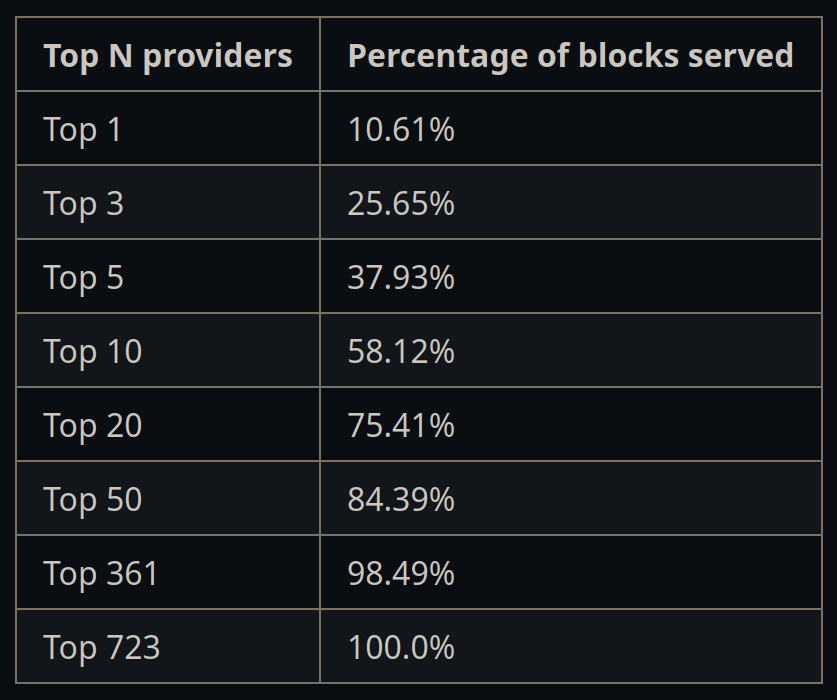
\includegraphics[width=\textwidth]{plots/top_provs.png}
    \end{center}
\end{column}
\begin{column}{0.64\textwidth}
    \begin{center}
		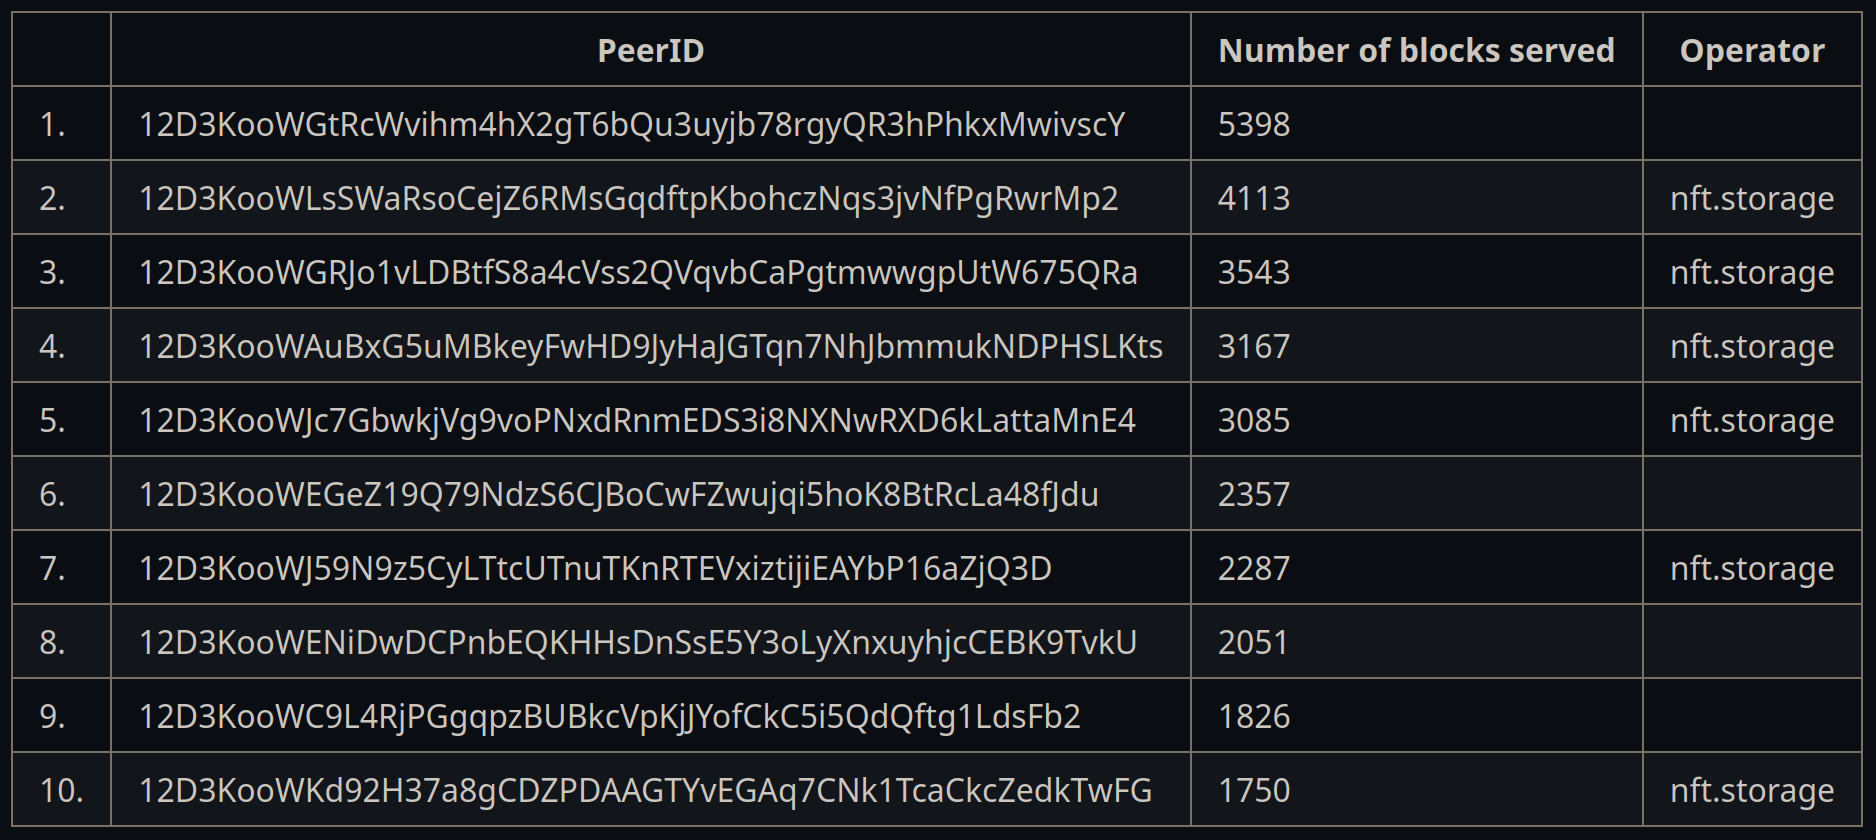
\includegraphics[width=\textwidth]{plots/top10.png}
    \end{center}
\end{column}
\end{columns}
\end{frame}

\begin{frame}
\frametitle{Bitswap Discovery + Fetch Latencies}
\begin{columns}[onlytextwidth]
\begin{column}{0.49\textwidth}
    \begin{center}
		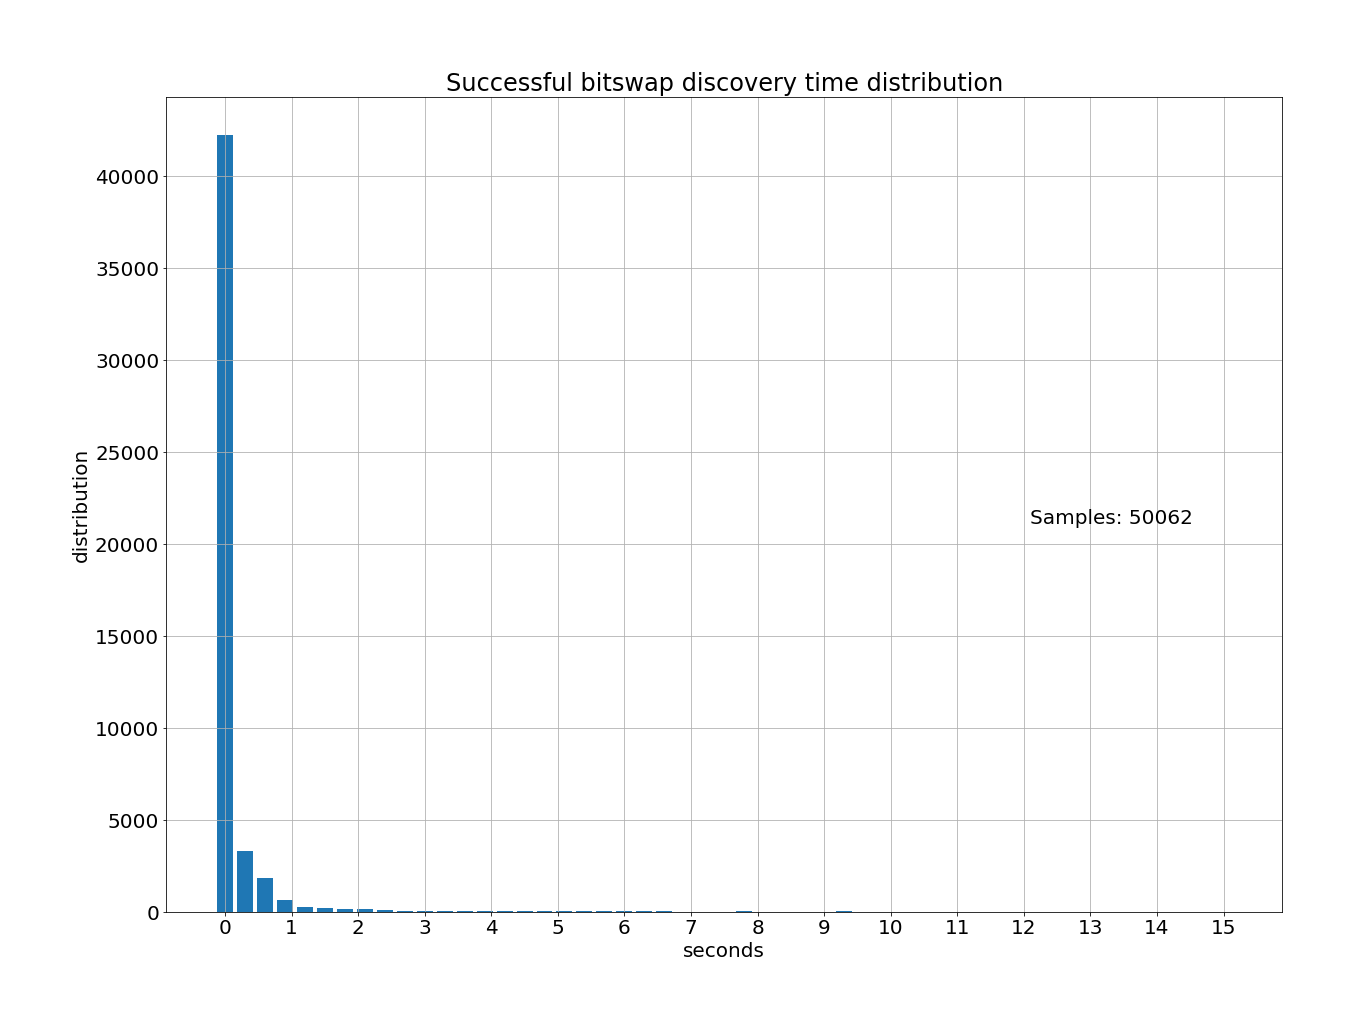
\includegraphics[width=\textwidth]{plots/pdf15.png}
    \end{center}
\end{column}
\begin{column}{0.49\textwidth}
    \begin{center}
		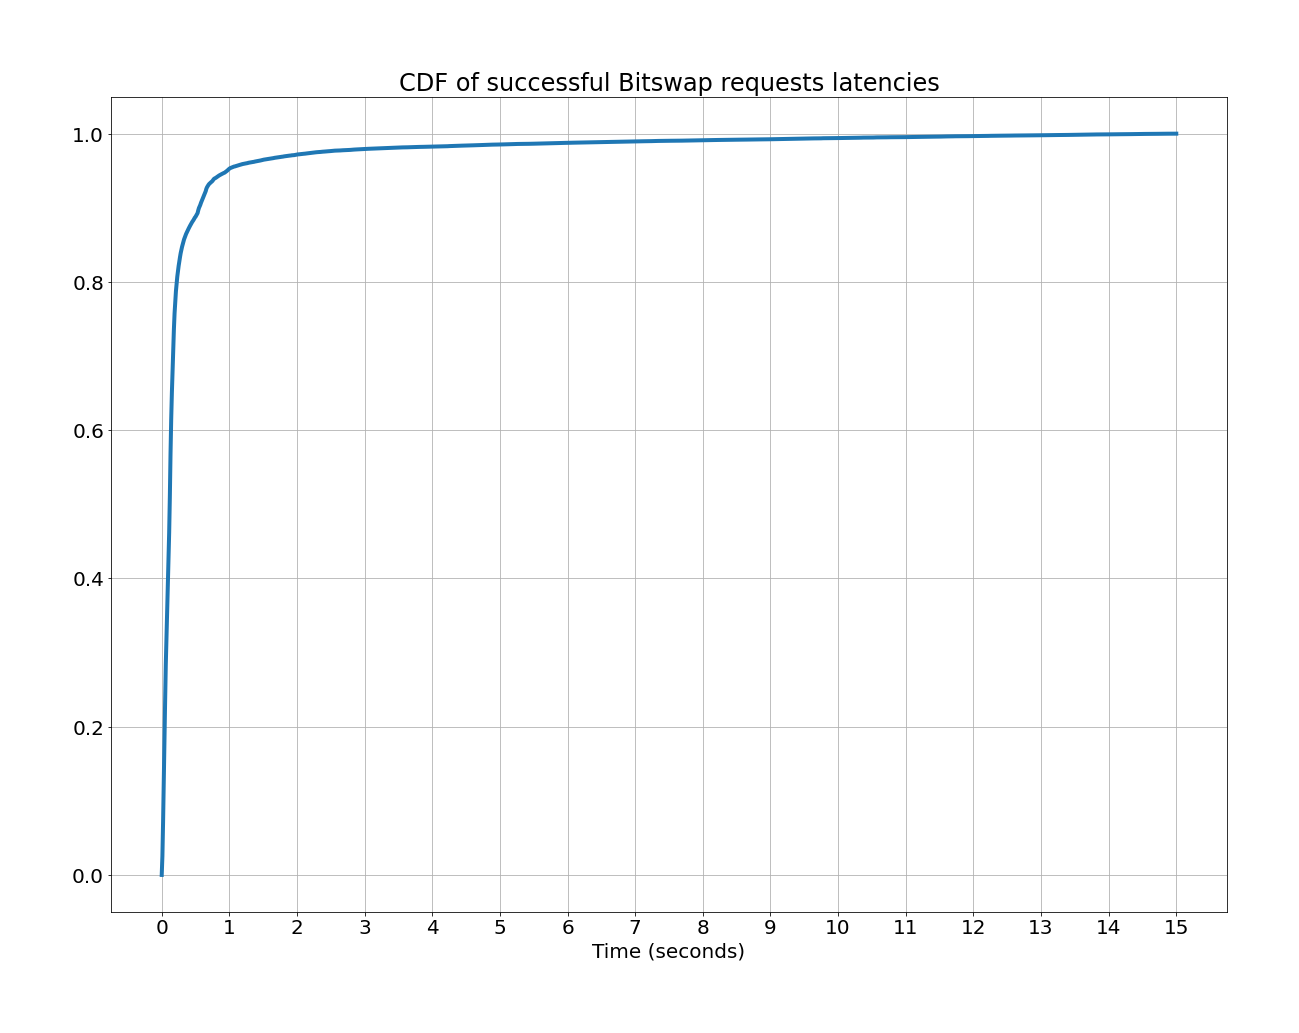
\includegraphics[width=\textwidth]{plots/cdf15.png}
    \end{center}
\end{column}
\end{columns}

\end{frame}

\begin{frame}
\frametitle{Bitswap Discovery + Fetch Latencies Zoom}
\begin{columns}[onlytextwidth]
\begin{column}{0.49\textwidth}
    \begin{center}
		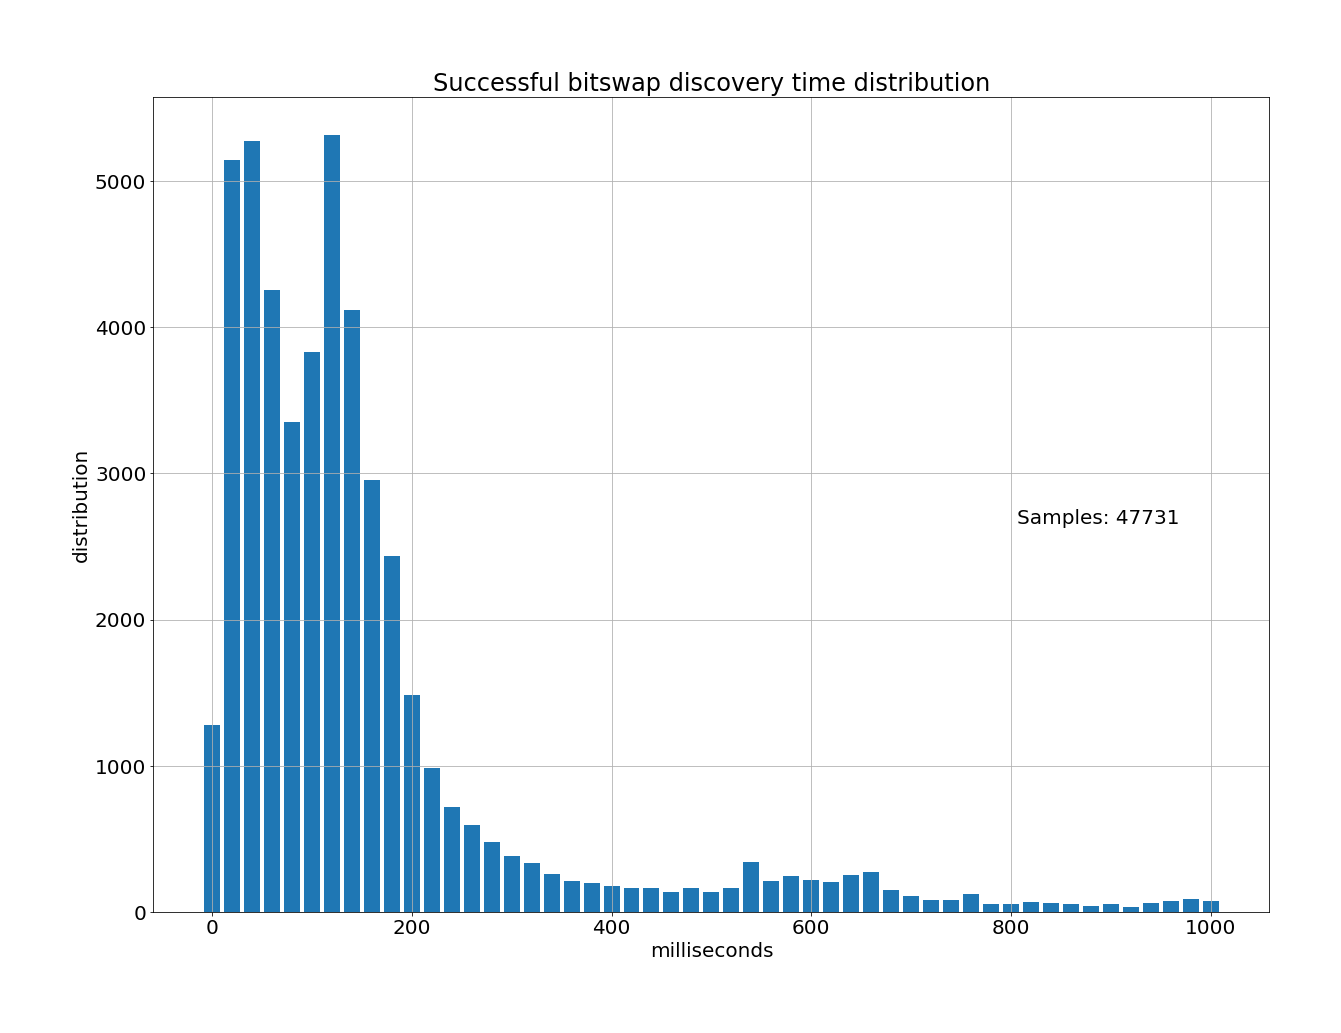
\includegraphics[width=\textwidth]{plots/pdf1.png}
    \end{center}
\end{column}
\begin{column}{0.49\textwidth}
    \begin{center}
		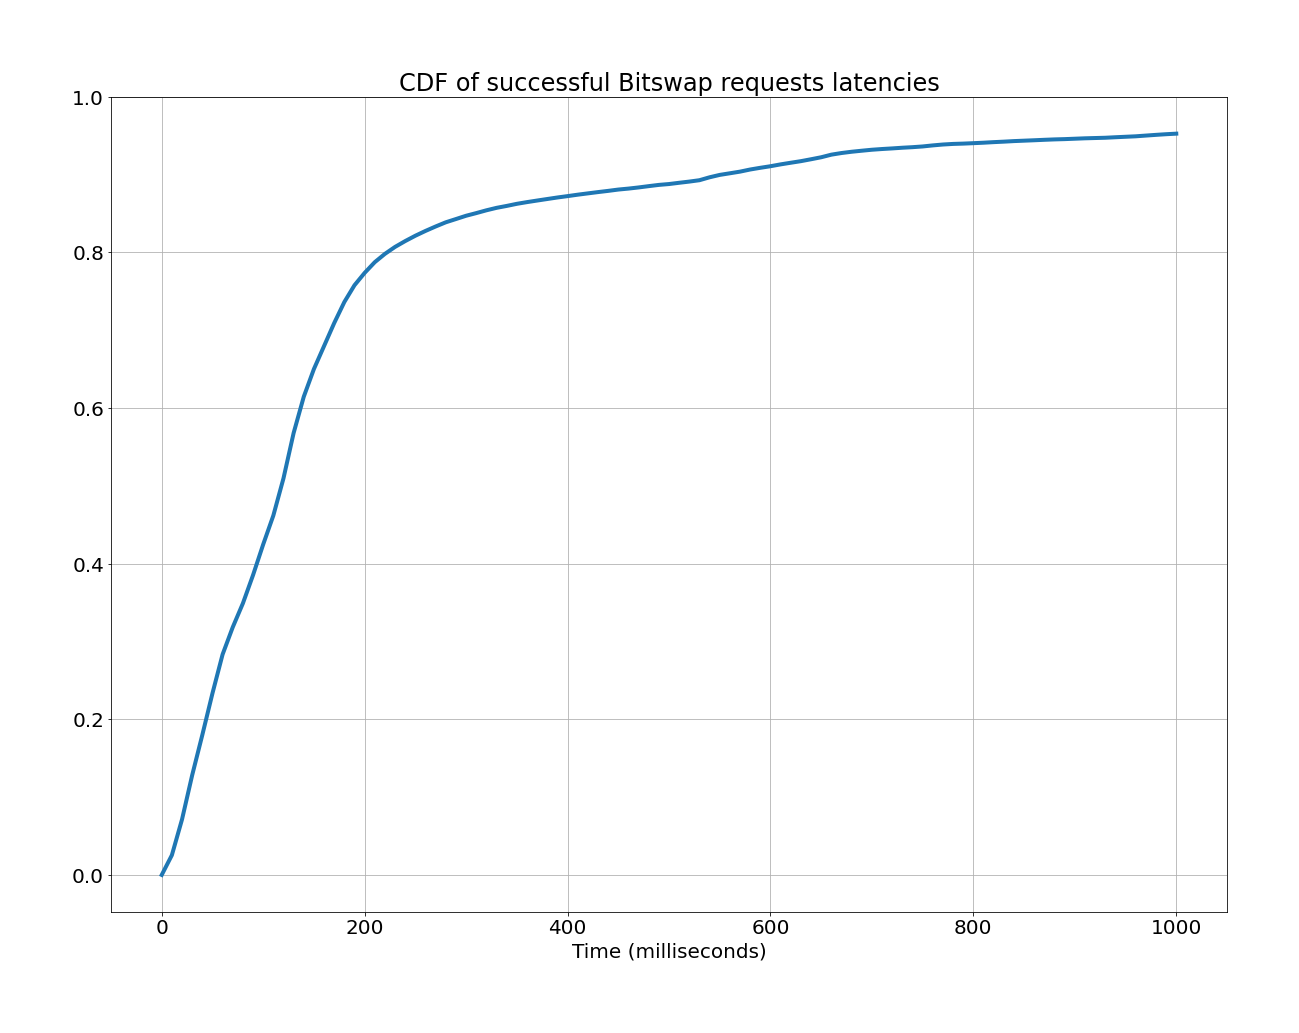
\includegraphics[width=\textwidth]{plots/cdf1.png}
    \end{center}
\end{column}
\end{columns}
\end{frame}

\begin{frame}
\frametitle{Takeaways}
\begin{itemize}
	\itemc Bitswap is currently \textbf{fast} (discovery+fetch $\leq 200$ms in $80\%$) and \textbf{accurate} ($98.37\%$ of accessible content found)
	\itemc Bitswap is \textbf{inefficient} ($856$ peers solicited for each request)
	\itemc Bitswap content discovery \textbf{does NOT scale} (e.g if the network grows by 10x, the number of open connection must be 10x to keep the same discovery success rate)
	\itemc The top 20 peers serve $75\%$ of the requested content
	\bigskip
	\itemc Should data transfer and content routing be bundled together?
\end{itemize}
\end{frame}

\begin{frame}
\frametitle{References}
\begin{columns}[onlytextwidth]
\begin{column}{0.60\textwidth}
\begin{itemize}
	\itemc Detailed report
	\itemc Complete measurement methodology
	\itemc Additional data and plots
	\itemc Improvement recommendations
\end{itemize}
\end{column}
\begin{column}{0.38\textwidth}
\begin{center}
\qrcode[height=4cm]{https://github.com/guillaumemichel/network-measurements-rfm16/blob/master/results/rfm16-bitswap-discovery-effectiveness.md}\\
\medskip
RFM-16 Report
\bigskip
\end{center}
\end{column}
\end{columns}

\begin{itemize}
	\itemc Soon available at\hspace{.6em}\url{https://github.com/protocol/network-measurements}

\end{itemize}

\end{frame}


\end{document}